\documentclass[11pt,a4paper]{article}
\usepackage[T1]{fontenc}
\usepackage[utf8]{inputenc}
\usepackage[margin=2.15cm]{geometry}
\usepackage{setspace}
\setstretch{1.08}
\usepackage{amsmath,amssymb}
\usepackage{graphicx}
\usepackage{booktabs}
\usepackage{tikz}
\usetikzlibrary{arrows.meta,positioning}
\usepackage[hidelinks]{hyperref}
\newcommand{\vect}[1]{\mathbf{#1}}
\graphicspath{{../paper/figs/}}
\setlength{\parskip}{0.32em}
\setlength{\parindent}{1.15em}

\title{\textbf{A Modified Shuffled Frog-Leaping Search\\ for an SVM Fault Classifier}}
\author{Short paper on the second innovation of the expanded study\\
based on You, Fan, Li, Liang, Fang, and Wang,\\
\textit{Shock and Vibration}, 2019, Article ID 1908485}
\date{}

\begin{document}
\maketitle
\thispagestyle{empty}
\vspace{-1.6em}

\begin{abstract}
\noindent
A radial-basis support vector machine separates the $22$-dimensional vibration features of a four-state pump only after two numbers are chosen: the soft-margin penalty $C$ and the kernel parameter $g$.
Cross-validated accuracy, the natural score of a candidate pair, is a step function, so the outer search has to be derivative-free.
Shuffled frog-leaping already mixes a local leap toward the best frog in a memeplex with a later leap toward the best frog in the population, and it replaces a failed frog by a uniform draw.
That cascade wastes a training whenever both leaders would have helped at once, and the uniform draw abandons a position the search has already paid for.
The modification makes one leap, with weights set by distance to the global best, and replaces a failure by a Gaussian perturbation of the current frog in logarithmic coordinates.
On the published split, $180$ training vectors and $60$ test vectors, the modified search labels $56$ test vectors correctly.
The unmodified frog-leaping search and a chemical-reaction search each label $55$.
A backpropagation network labels $51$.
The gain over the other global searches is one test vector, and it is reported as a count.
\end{abstract}

\section{The classifier the search is wrapped around}

The feature vector is fixed before this innovation begins.
Each record has already been reduced to $\vect{x}\in\mathbb{R}^{22}$ and scaled to the unit interval on training ranges.
The label set has four states: healthy, eccentric axle, bearing pedestal, and sealing-ring wear.
Binary soft-margin machines are the decision rule \cite{cortes1995,vapnik1995}.
With labels $y_i\in\{+1,-1\}$ the dual used here is
\begin{equation}
\begin{aligned}
\min_{\alpha}\;&
\frac12\sum_{i,j} y_i y_j \alpha_i \alpha_j
\Bigl(K(\vect{x}_i,\vect{x}_j)+\frac{1}{C}\delta_{ij}\Bigr)
-\sum_j \alpha_j\\
\text{s.t.}\;&
\sum_i y_i\alpha_i=0,\qquad \alpha_i\ge 0,
\end{aligned}
\label{eq:dual}
\end{equation}
and the decision value is $\sum_i \alpha_i y_i K(\vect{x},\vect{x}_i)+b$.
The radial kernel
\begin{equation}
K(\vect{x},\vect{x}')=\exp\bigl(-g\,\lVert\vect{x}-\vect{x}'\rVert^{2}\bigr),
\qquad g=1/(2\sigma^{2}),
\label{eq:rbf}
\end{equation}
is positive definite for every $g>0$ \cite{scholkopf2002}.
A large $C$ punishes slacks and can memorize $180$ rows.
A large $g$ makes $K$ local and can do the same.
The pair $(C,g)$ is the whole continuous freedom of the classifier \cite{hsu2003,widodo2007}.

Four states are reduced by one-versus-one voting: six binary machines, each trained on the $90$ rows of one pair of states.
One shared pair $(C,g)$ is used for all six.
The search works in logarithmic coordinates $\vect{u}=(\log_{10} C,\log_{10} g)$ inside the box $\log_{10} C\in[-1,3]$ and $\log_{10} g\in[-3,1]$.
The 2019 paper does not print the box; the rectangle is the specification that makes a leap a multiplicative step.
Fitness is stratified five-fold accuracy of the voted label on the $180$ training rows.
The $60$ test rows are used once, after the best frog is retrained on all $180$.

\section{The unmodified leap and its two defects}

A frog is a candidate $\vect{u}$.
The population is sorted by fitness and dealt round-robin into memeplexes, so each memeplex receives a high-fitness frog \cite{eusuff2003,eusuff2006}.
Inside a memeplex the worst frog $\vect{F}_{w}$ first steps toward the local best $\vect{F}_{b}$,
\begin{equation}
\vect{D}=\mathrm{rand}(0,1)\,(\vect{F}_{b}-\vect{F}_{w}),
\qquad
\vect{F}_{w}^{\mathrm{new}}=\mathrm{clip}(\vect{F}_{w}+\vect{D}).
\label{eq:cascade}
\end{equation}
Only if that step fails to raise fitness does the same formula replace $\vect{F}_{b}$ by the global best $\vect{F}_{g}$.
If that also fails, $\vect{F}_{w}$ is replaced by a uniform draw in the box.
The clip enforces the box and a maximum step.
Two defects follow from the formulae.
The two leaders are never used in the same step, so a frog that needs a mixture of them spends a full cross-validated training to discover that the first leader was not enough.
And a failed frog is thrown away.
Late in the run, when frogs already agree, both defects shrink the diversity the shuffle was meant to protect \cite{you2019}.

\section{The modified leap}

Let $\vect{U}_{z,c}$ be the mean position of memeplex $z$.
Distance between frogs $i$ and $j$ adds the distance of those centers to the Euclidean distance of the frogs, so two memeplexes that have drifted apart are not treated as neighbors merely because two members happen to lie close.
Write $D_{\max}^{g}$ and $D_{\min}^{g}$ for the greatest and least such distances from any other frog to the global best.
The weights on the two leaders are
\begin{equation}
q=\frac{\mathrm{dist}(i,\vect{F}_{g})-D_{\min}^{g}}{D_{\max}^{g}-D_{\min}^{g}},
\qquad h=1-q,
\label{eq:hq}
\end{equation}
and $h=q=\tfrac12$ if every distance is equal.
A frog near the global best gets a large $h$ and mostly follows its memeplex.
A frog far from the global best gets a large $q$ and is pulled inward without waiting for a failed local try.
The step is the single update
\begin{equation}
\begin{aligned}
\vect{D}
&=h\,\mathrm{rand}(0,1)\,(\vect{F}_{b}-\vect{F}_{w})
+q\,\mathrm{rand}(0,1)\,(\vect{F}_{g}-\vect{F}_{w}),\\
\vect{F}_{w}^{\mathrm{new}}
&=\mathrm{clip}(\vect{F}_{w}+\vect{D}).
\end{aligned}
\label{eq:leap}
\end{equation}
The two random factors are independent and have mean one half, so the expected step is
\begin{equation}
\mathbb{E}[\vect{D}]
=\frac{h}{2}(\vect{F}_{b}-\vect{F}_{w})+\frac{q}{2}(\vect{F}_{g}-\vect{F}_{w}).
\label{eq:mean}
\end{equation}
Distance selects the mixture before fitness is spent.
If the new fitness is not strictly better, the frog is mutated in place,
\begin{equation}
\vect{F}_{w}^{\mathrm{mut}}
=\mathrm{clip}\bigl(\vect{F}_{w}+\vect{F}_{w}\odot\boldsymbol{\varepsilon}\bigr),
\qquad \boldsymbol{\varepsilon}\sim\mathcal{N}(\vect{0},\vect{I}),
\label{eq:gauss}
\end{equation}
instead of being redrawn uniformly.
Because the coordinates are logarithms, adding a multiple of the coordinate is a multiplicative jitter of $C$ and of $g$.
A unit normal draw of size $0.2$ changes $C$ by a factor of about $10^{0.36}\approx 2.3$.
That is large enough to leave a flat step of the accuracy surface and small enough to remain a neighbor.
The mutant is accepted even if it is worse, which is what restores diversity, and the clip is what stops a wild Gaussian draw from becoming the old uniform restart.

\begin{figure}[ht]
\centering
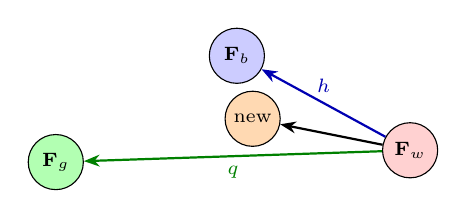
\begin{tikzpicture}[
  f/.style={circle, draw, inner sep=1.2pt, font=\scriptsize, minimum size=7mm},
  arr/.style={-{Stealth[length=2mm]}, thick}]
\node[f, fill=green!30] (g) at (0,0) {$\vect{F}_{g}$};
\node[f, fill=blue!20] (b) at (2.3,1.35) {$\vect{F}_{b}$};
\node[f, fill=red!18] (w) at (4.5,0.15) {$\vect{F}_{w}$};
\node[f, fill=orange!30] (n) at (2.5,0.55) {new};
\draw[arr, blue!70!black] (w)--(b) node[midway, above, font=\scriptsize] {$h$};
\draw[arr, green!50!black] (w)--(g) node[midway, below, font=\scriptsize] {$q$};
\draw[arr] (w)--(n);
\end{tikzpicture}
\caption{One leap uses the local best and the global best together. The weights $h$ and $q$ depend on distance to the global best. A failed leap is a Gaussian mutation of $\vect{F}_{w}$, not a uniform restart.}
\label{fig:leap}
\end{figure}

The outer loop is then: draw a population in the box; score it; deal memeplexes; repeat the leap-or-mutate step; shuffle; stop at a fixed budget or at a fitness target; retrain the six machines on all $180$ rows at the returned pair; label the test rows by vote.
Population size and shuffle count are not printed in the source study and are not reconstructed here.
A software starting point is five memeplexes of ten frogs, ten local steps, and thirty shuffles, which is about $1550$ fitness evaluations and $30$ binary trainings per evaluation.
That schedule is a suggestion, not a claim about the 2019 run.

\section{The published count}

All four methods in the comparison read the same VWC vectors \cite{you2019}.
They differ in the map from vector to label.
The backpropagation network has no $(C,g)$ \cite{huang2009}.
ACROA-SVM wraps a chemical-reaction search around the same dual \cite{ao2014,alatas2011}.
SFLA-SVM uses the cascade \eqref{eq:cascade}.
MSFLA-SVM uses \eqref{eq:leap} and \eqref{eq:gauss}.
Table~\ref{tab:err} gives error counts.
Training errors are out of $180$.
Test errors are out of $60$, and the class columns are out of $15$.

\begin{table}[ht]
\centering
\caption{Error counts on the published split. The BPNN sealing-ring test count is the count consistent with the printed percentage and the printed $85\%$ pooled accuracy.}
\label{tab:err}
\begin{tabular}{lrrrrrr}
\toprule
Method & Train & Test & Normal & EAF & BPF & SRWF \\
\midrule
BPNN & 15 & 9 & 2 & 2 & 3 & 2 \\
ACROA-SVM & 5 & 5 & 0 & 2 & 2 & 1 \\
SFLA-SVM & 6 & 5 & 0 & 1 & 2 & 2 \\
MSFLA-SVM & 3 & 4 & 0 & 1 & 2 & 1 \\
\bottomrule
\end{tabular}
\end{table}

\begin{figure}[ht]
\centering
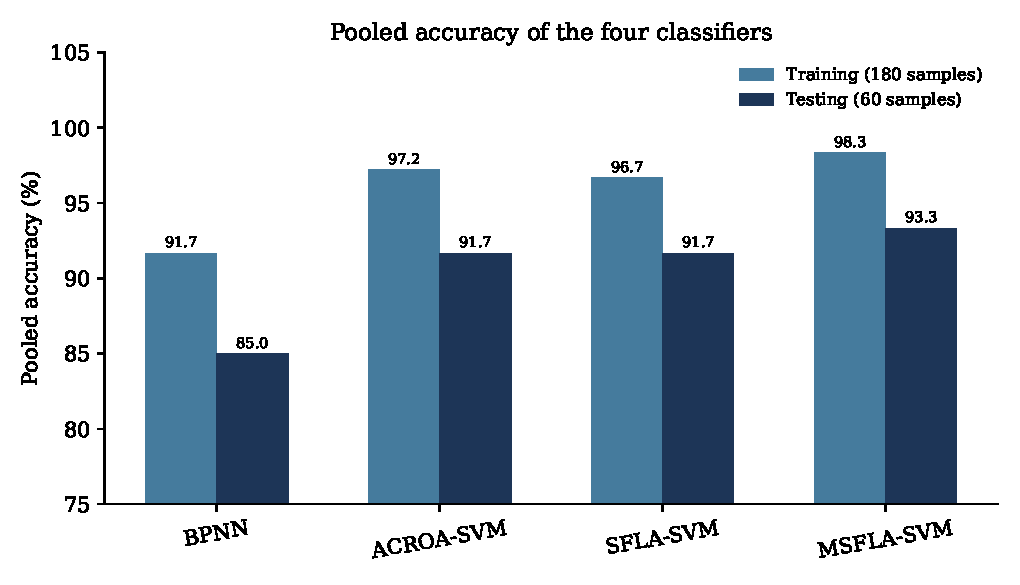
\includegraphics[width=0.78\textwidth]{pooled_accuracy.pdf}
\caption{Pooled accuracy. The modified search is highest on both the training rows and the test rows. The test margin over each other SVM search is one vector.}
\label{fig:pool}
\end{figure}

MSFLA-SVM is never behind SFLA-SVM on a test class.
The entire pooled test gain is one sealing-ring vector: $14/15$ against $13/15$.
On the pedestal class every SVM method misses two of fifteen.
The modification collects, in one rule, the eccentric count of the unmodified leap and the seal-wear count of the chemical-reaction search.
It does not buy a pedestal test vector.
The train-to-test drop is $5.0$ points for both frog-leaping machines and $6.7$ points for the neural baseline, so the higher training accuracy of the modified search is not paid for by a larger drop.
A one-vector gap on a sixty-vector test set is the smallest nonzero gap the experiment can print.
It supports the claim that the modified leap is not worse than the two other global searches.
It is thin evidence that the leap is largely better.
Five test vectors against the neural baseline, nine errors against four, is the larger and more stable difference, and it belongs to the margin machine as a class, not only to the modification.

\section{Conclusion}

The second innovation leaves the support vector machine and its radial kernel unchanged and changes the proposal of $(C,g)$.
Every leap learns from the local best and the global best with weights set by distance, and every failed leap mutates the current frog instead of restarting.
On the published pump split the resulting classifier makes four test errors.
The unmodified leap and the chemical-reaction search make five each.
The pedestal class remains at two test errors for every SVM method, which locates the open problem in the feature and in the interference, not in a further tweak of the same two parameters.

\begin{thebibliography}{9}
\bibitem{you2019}
L.~You, W.~Fan, Z.~Li, Y.~Liang, M.~Fang, and J.~Wang,
``A fault diagnosis model for rotating machinery using VWC and MSFLA-SVM based on vibration signal analysis,''
\textit{Shock and Vibration}, vol.~2019, Article ID 1908485, 2019.
\bibitem{cortes1995}
C.~Cortes and V.~Vapnik,
``Support-vector networks,''
\textit{Machine Learning}, vol.~20, no.~3, pp.~273--297, 1995.
\bibitem{vapnik1995}
V.~N.~Vapnik,
\textit{The Nature of Statistical Learning Theory}.
New York: Springer, 1995.
\bibitem{eusuff2003}
M.~M.~Eusuff and K.~E.~Lansey,
``Optimization of water distribution network design using the shuffled frog leaping algorithm,''
\textit{J.\ Water Resources Planning and Management}, vol.~129, no.~3, pp.~210--225, 2003.
\bibitem{eusuff2006}
M.~Eusuff, K.~Lansey, and F.~Pasha,
``Shuffled frog-leaping algorithm: a memetic meta-heuristic for discrete optimization,''
\textit{Engineering Optimization}, vol.~38, no.~2, pp.~129--154, 2006.
\bibitem{hsu2003}
C.-W.~Hsu, C.-C.~Chang, and C.-J.~Lin,
``A practical guide to support vector classification,''
Technical report, National Taiwan University, 2003.
\bibitem{widodo2007}
A.~Widodo and B.-S.~Yang,
``Support vector machine in machine condition monitoring and fault diagnosis,''
\textit{Mechanical Systems and Signal Processing}, vol.~21, no.~6, pp.~2560--2574, 2007.
\bibitem{scholkopf2002}
B.~Sch\"olkopf and A.~J.~Smola,
\textit{Learning with Kernels}.
Cambridge, MA: MIT Press, 2002.
\bibitem{huang2009}
Z.~G.~Huang and Y.~Xie,
``Fault diagnosis method of rolling bearing based on BP neural network,''
in \textit{Proc.\ ICMTMA}, pp.~647--649, 2009.
\bibitem{ao2014}
H.~L.~Ao, J.~S.~Cheng, K.~L.~Li, and T.~K.~Truong,
``A roller bearing fault diagnosis method based on LCD energy entropy and ACROA-SVM,''
\textit{Shock and Vibration}, vol.~2014, Article ID 825825, 2014.
\bibitem{alatas2011}
B.~Alatas,
``ACROA: Artificial chemical reaction optimization algorithm for global optimization,''
\textit{Expert Systems with Applications}, vol.~38, no.~10, pp.~13170--13180, 2011.
\end{thebibliography}

\end{document}
